\chapter{Eksperimen dan Pembangunan Sistem}

\section{Lingkungan Eksperimen dan Pembangunan Sistem}

Eksperimen dilakukan di platform \href{https://www.kaggle.com}{Kaggle} dengan Kernel gratisnya. Bahasa Pemrograman yang digunakan adalah bahasa Python versi 3.6.6 dan CPU 1xSingle core hyper threaded Xeon Processors @2.3Ghz, 46MB Cache.

Untuk memastikan bahwasanya eksperimen \textit{reproducible} dan tidak memiliki faktor acak, semua opsi \textit{seed} baik di System, Python, hingga pustaka Pytorch ditetapkan agar hasil tidak berubah jika eksperimen dijalankan berkali-kali dengan kondisi yang sama.

\begin{lstlisting}[language=Python]
def set_seed():
    seed=1
    random.seed(seed)
    torch.manual_seed(seed)
    torch.cuda.manual_seed_all(seed)
    np.random.seed(seed)
    os.environ['PYTHONHASHSEED'] = str(seed)
    torch.backends.cudnn.deterministic = True
\end{lstlisting}



\section{Eksperimen}
Secara keseluruhan, eksperimen yang dilakukan adalah dengan 2 model cross-lingual language model (XLM-R \& Multilingual BERT), 2 dataset sentimen Bahasa Indonesia (TripAdvisor \& Prosa), 2 bahasa transfer (Bahasa Inggris dan Bahasa Malaysia). Eksperimen antar model XLM-R dan Multilingual BERT dapat memperlihatkan kemajuan yang XLM-R dapatkan dengan menggunakan subword dan data lebih banyak. Dalam kedua kasus, XLM-R dan Multilingual BERT tidak dilatih ulang, melainkan model yang ada sekarang digunakan untuk mengekstraksi fitur dari teks. Teks kemudian dimasukkan ke sebuah layer neural network yang dilatih.

Selain itu, eksperimen juga dicoba dengan total data divariasikan (100 / 250 / 500 / 750 / 1000 / 2500 / 5000 / 7500 / 10981 (10000 jika TripAdvisor) / (12389 jika TripAdvisor)) dan total banyak data transfer divariasikan juga (1x - 10x). Dengan hal ini, dapat dibandingkan efek \textit{cross-lingual language model} antar banyak jumlah data dan juga antar banyaknya jumlah data transfer.

\textbf{\textcolor{red}{Subbab berikutnya baru menampilkan plot hasil eksperimen. Teks yang menjelaskan akan diisi secepatnya.}}

    \subsection{Dataset Prosa, Model XLM-R. dan Bahasa Inggris Sebagai Bahasa Transfer}
        Berikut hasil eksperimen: 
        \begin{figure}[ht]
            \centering
            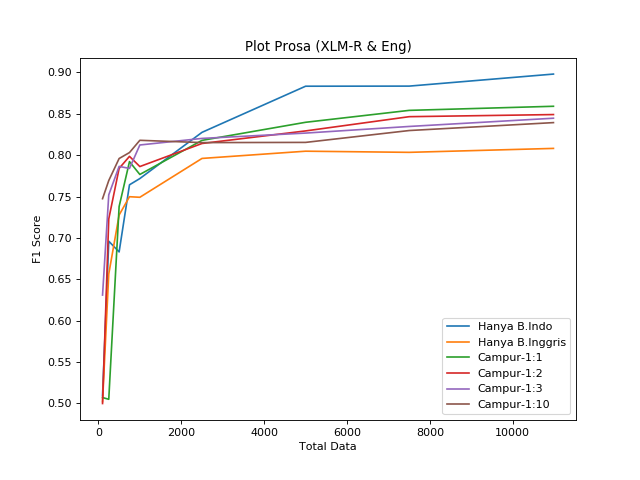
\includegraphics[width=0.75\textwidth]{resources/prosa-xlmr-eng-1.png}
            \caption{Plot antara f1-score dan total data pada eksperimen dataset Prosa dengan model XLM-R dan Bahasa Inggris sebagai bahasa transfer.}

            \label{fig:prosa_xlmr_eng_1}
        \end{figure}

        \begin{figure}[ht]
            \centering
            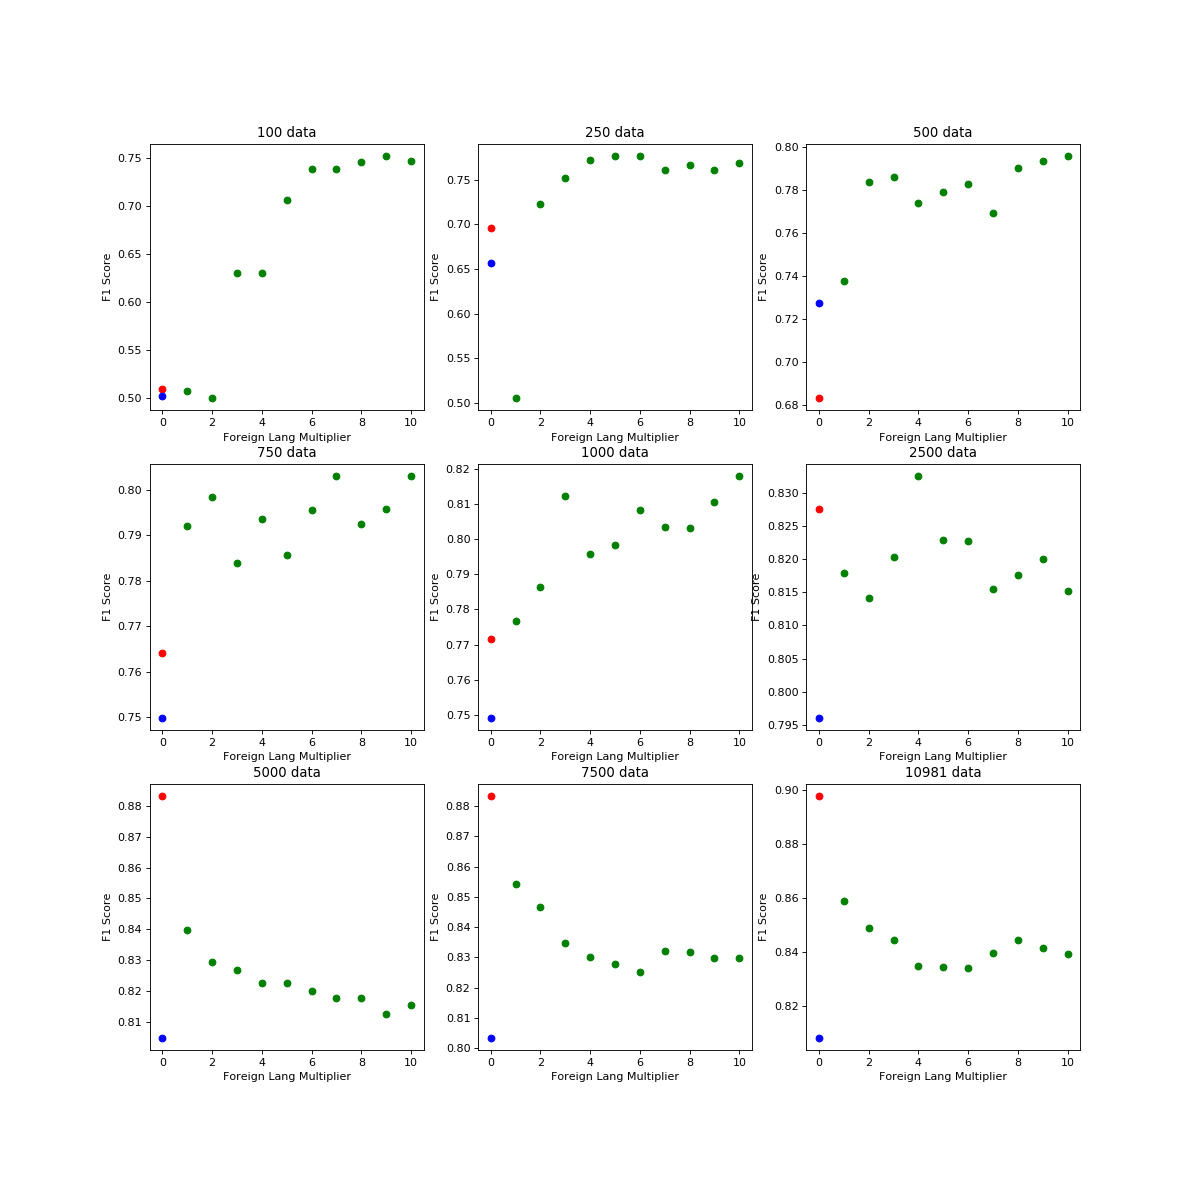
\includegraphics[width=0.75\textwidth]{resources/prosa-xlmr-eng-2.png}
            \caption{Plot antara total data dan banyaknya kelipatan bahasa transfer pada eksperimen dataset Prosa dengan model XLM-R dan Bahasa Inggris sebagai bahasa transfer.}

            \label{fig:prosa_xlmr_eng_2}
        \end{figure}


    \subsection{Dataset Prosa, Model XLM-R dan Bahasa Malaysia Sebagai Bahasa Transfer}
        Berikut hasil eksperimen: 
        \begin{figure}[ht]
            \centering
            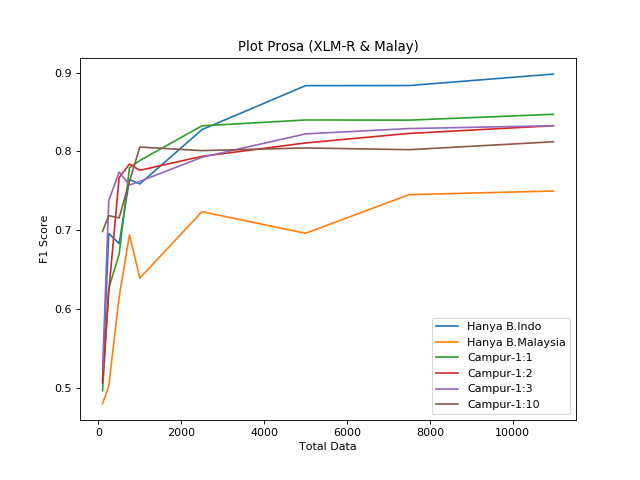
\includegraphics[width=0.75\textwidth]{resources/prosa-xlmr-malay-1.png}
            \caption{Plot antara f1-score dan total data pada eksperimen dataset Prosa dengan model XLM-R dan Bahasa Malaysia sebagai bahasa transfer.}

            \label{fig:prosa_xlmr_malay_1}
        \end{figure}

        \begin{figure}[ht]
            \centering
            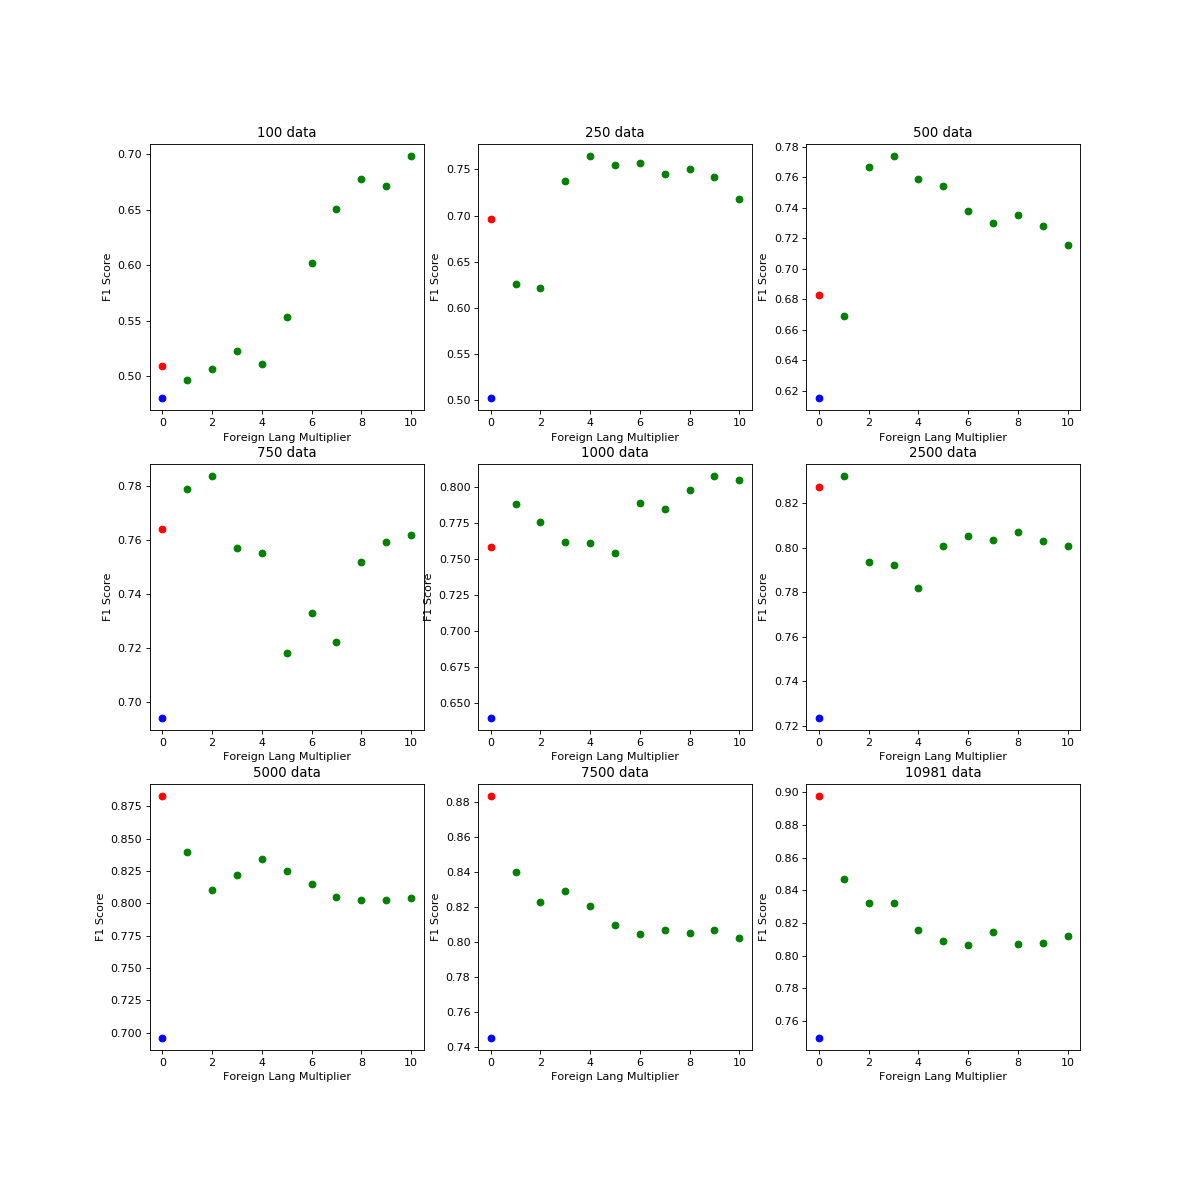
\includegraphics[width=0.75\textwidth]{resources/prosa-xlmr-malay-2.png}
            \caption{Plot antara total data dan banyaknya kelipatan bahasa transfer pada eksperimen dataset Prosa dengan model XLM-R dan Bahasa Malaysia sebagai bahasa transfer.}

            \label{fig:prosa_xlmr_malay_2}
        \end{figure}

    \subsection{Dataset Prosa, Model Multilingual BERT dan Bahasa Inggris Sebagai Bahasa Transfer}
        Berikut hasil eksperimen: 
        \begin{figure}[ht]
            \centering
            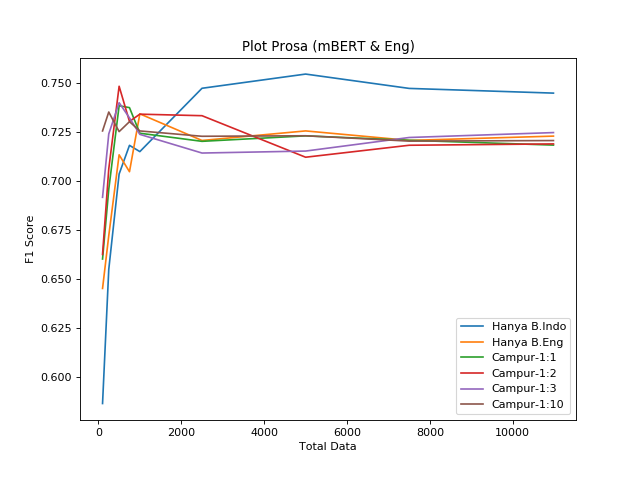
\includegraphics[width=0.75\textwidth]{resources/prosa-mbert-eng-1.png}
            \caption{Plot antara f1-score dan total data pada eksperimen dataset Prosa dengan model Multilingual BERT dan Bahasa Inggris sebagai bahasa transfer.}

            \label{fig:prosa_mbert_eng_1}
        \end{figure}

        \begin{figure}[ht]
            \centering
            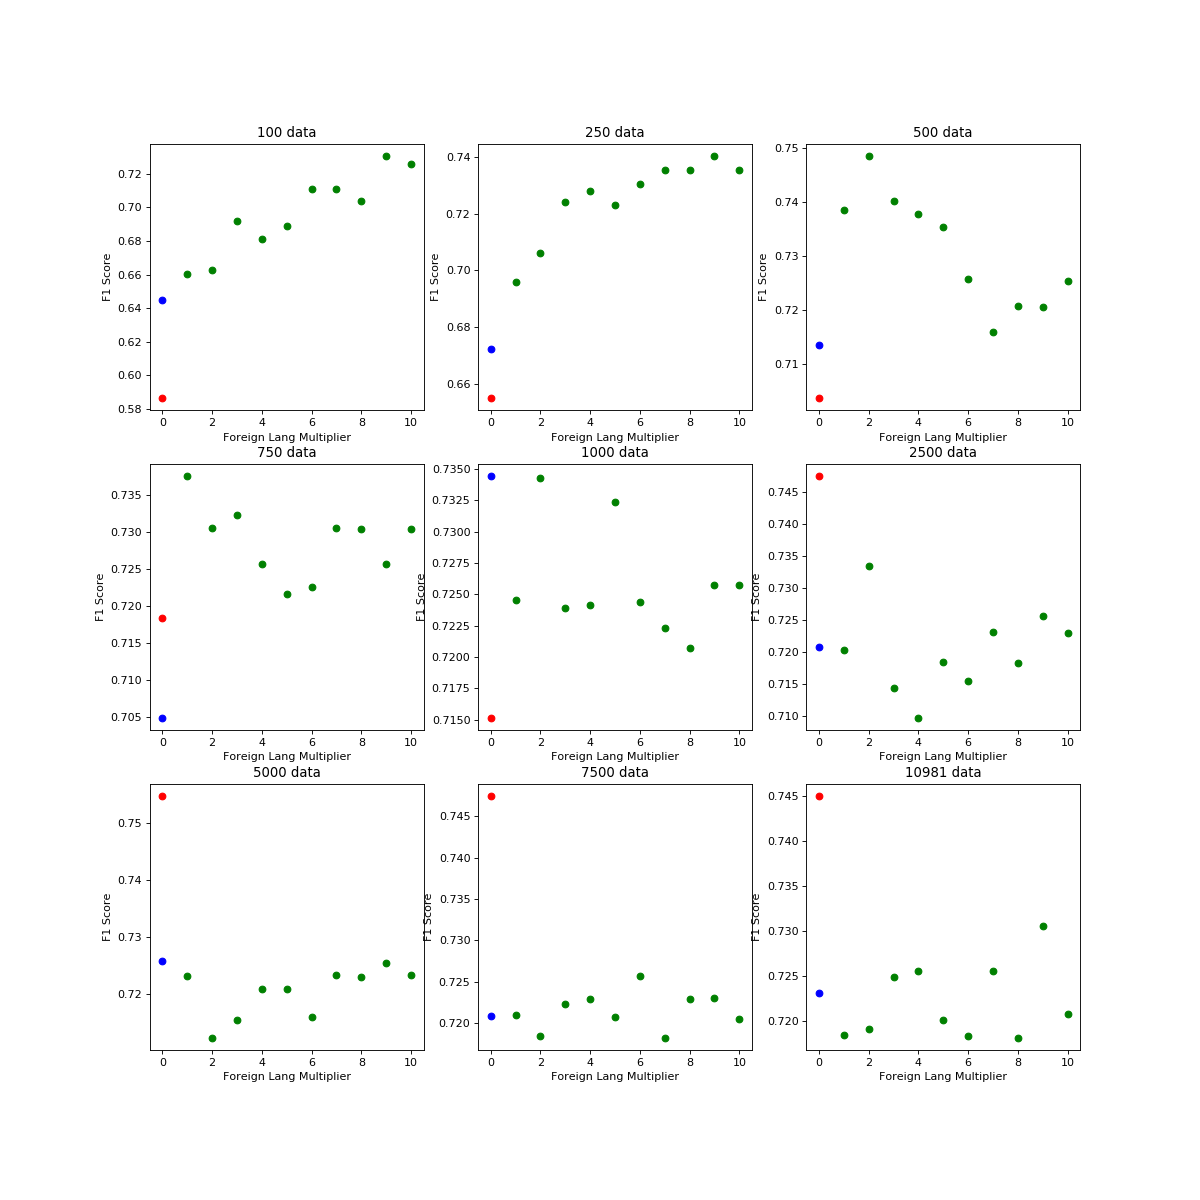
\includegraphics[width=0.75\textwidth]{resources/prosa-mbert-eng-2.png}
            \caption{Plot antara total data dan banyaknya kelipatan bahasa transfer pada eksperimen dataset Prosa dengan model Multilingual BERT dan Bahasa Inggris sebagai bahasa transfer.}

            \label{fig:prosa_mbert_eng_2}
        \end{figure}

    \subsection{Dataset Prosa, Model Multilingual BERT dan Bahasa Malaysia Sebagai Bahasa Transfer}

        Berikut hasil eksperimen: 
        \begin{figure}[ht]
            \centering
            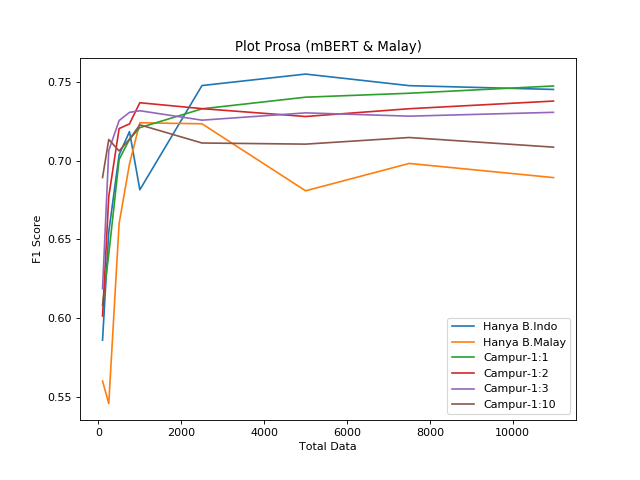
\includegraphics[width=0.75\textwidth]{resources/prosa-mbert-malay-1.png}
            \caption{Plot antara f1-score dan total data pada eksperimen dataset Prosa dengan model Multilingual BERT dan Bahasa Malaysia sebagai bahasa transfer.}

            \label{fig:prosa_mbert_malay_1}
        \end{figure}

        \begin{figure}[ht]
            \centering
            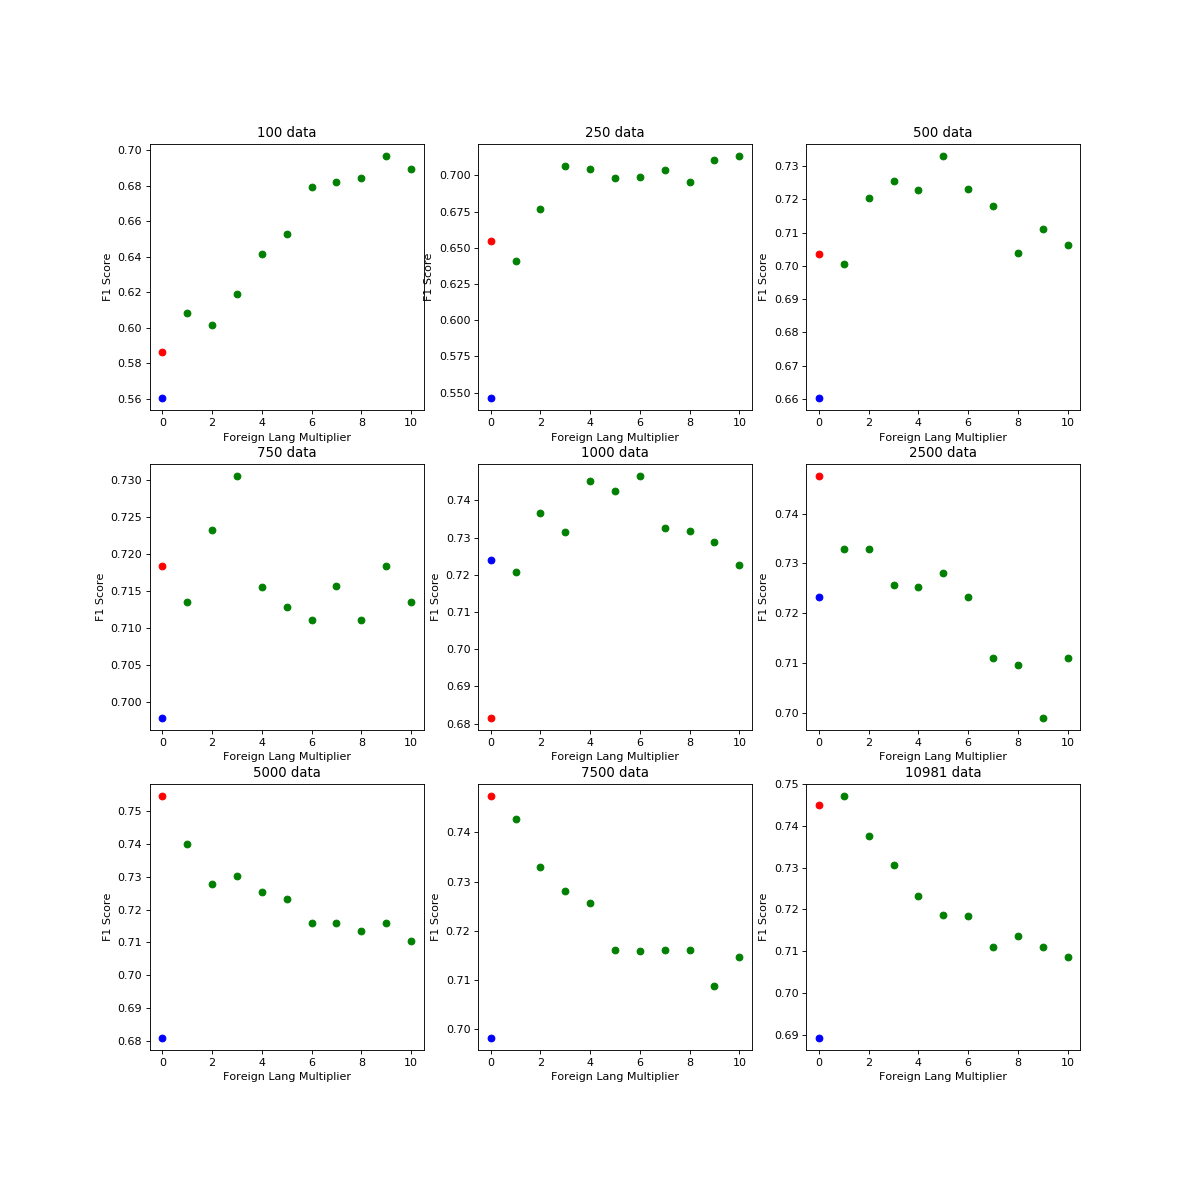
\includegraphics[width=0.75\textwidth]{resources/prosa-mbert-malay-2.png}
            \caption{Plot antara total data dan banyaknya kelipatan bahasa transfer pada eksperimen dataset Prosa dengan model Multilingual BERT dan Bahasa Malaysia sebagai bahasa transfer.}

            \label{fig:prosa_mbert_malay_2}
        \end{figure}
